\chapter{Developing an Effective Visualization of Conditional Probability} \label{app:devmob}

As noted in \ref{c:introduction} and \ref{sec:impactrace}, a
deficiency of the previous investigations of peremptory challenges
was a failure to generate compelling and effective visualizations of
the trends in the data. These investigations instead rely on tables to
communicate analysis. While such visualizations are not necessarily critical to analysis, they can often be incredibly useful to not only
communicate and compare data, but to motivate further investigations in a way which is clearer and more intuitive than
a simple table of values.

The first attempt at such a visualization was the mosaic plot (as discussed by \cite{friendly1994}) using the \texttt{mosaicplot}
function in the \texttt{graphics} package in R [\cite{Rcite}]. Figure \ref{fig:mosaicdefrace} displays this first approach with
disposition related to the simplified races of both the defendant and the venire member.

\begin{figure}[!h]
  \centering
  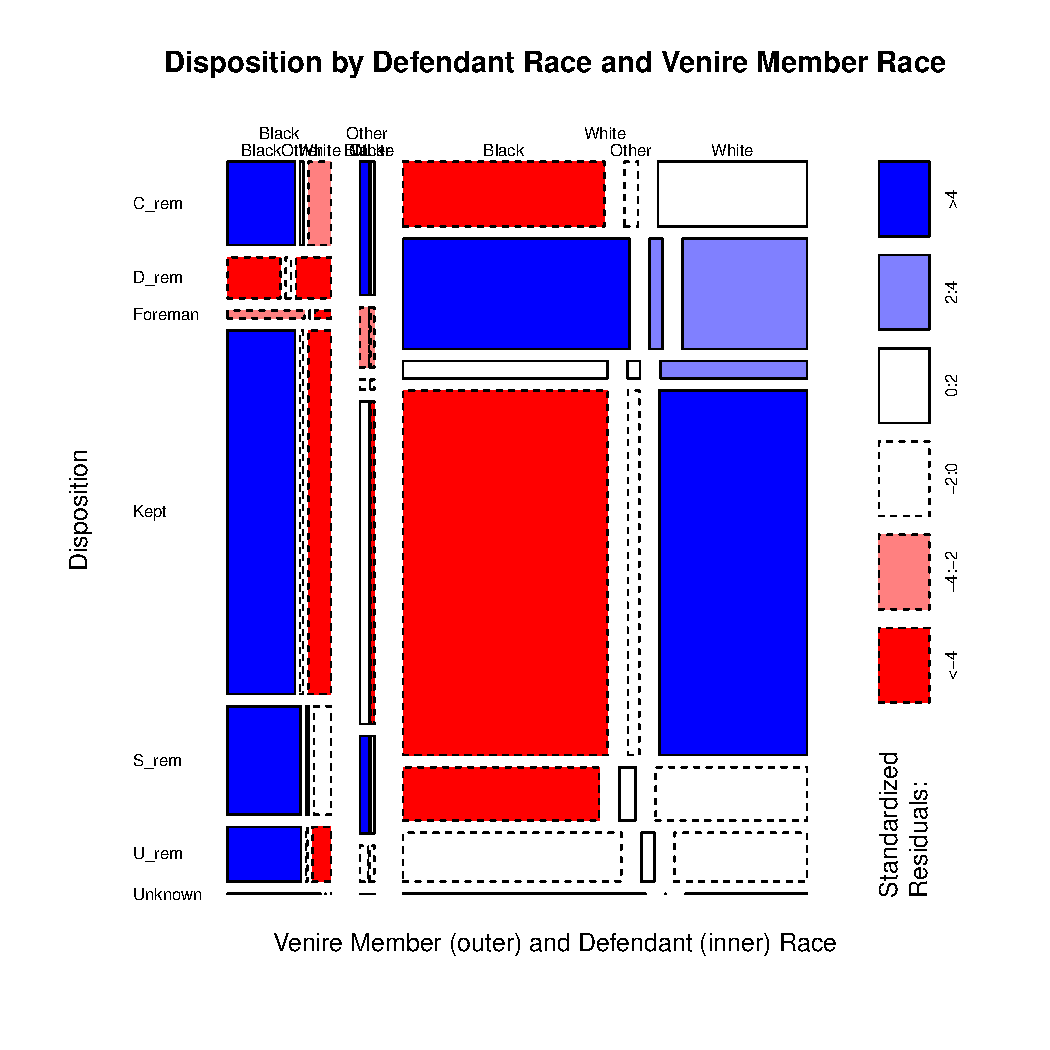
\includegraphics[width=0.7\textwidth]{Pictures/FirstMosaic}
  \caption[Mosaic Plot of Defendant and Venire Member
  Race]{\footnotesize A mosaic plot of the simplified defendant and venire member race and
    their relation to the disposition of the venire member.}
  \label{fig:mosaicdefrace}
\end{figure}

This visualization suffers from a number of limitations, some of which are obvious, and others of which are best explained by
the hierarchy of accuracy of visual perception provided in \cite{cleveland1987}. The obvious limitations are the lack of ability
to perceive the differences for the smallest groups, which are compressed enough that their shading is nearly
imperceptible. Additionally, the ordering of the axes is incredibly important in how the different areas appear visually, and
comparing the different areas is challenging as a result.

This is rather unsurprising. In ranking visual displays by accuracy of perception, \cite{cleveland1987} place area
low in the hierarchy. Areas are placed below angles, lengths, and positions along common scales. In \textit{The Visual Display of
  Quantitative Information}, \citeauthor{VisualDisplayQuant} gives two more sources of possible criticism of the mosaic plot as
displayed in Figure \ref{fig:mosaicdefrace}: the concept of data-ink and the dimensionality of visualization.

Of the mosaic plot, one may ask how much of the ``ink'', or structure, on the page is necessary to communicate the information
present. If one has a desire to ``above all else show the data'' as Tufte does, then these large shaded rectangles, which are
likely not perceived accurately according to \citeauthor{cleveland1987}, seem unnecessary compared to a simpler
visualization. This is the concept of ``data-ink,'' to reduce the complexity of the structures used to display the
data.

Hand-in-hand with this concept is \citeauthor{VisualDisplayQuant}'s rule that the dimensionality of a visualization should not be
larger than the data. In the case of the mosaic plot this is not strictly violated, as the marginal lengths used to create the
areas reflect a measurement of the data. Nonetheless, the areas of each rectangle correspond to a simple count in a contingency
table, and perhaps an area is not the best way to represent such a singular value.

\begin{figure}[!h]
  \centering
  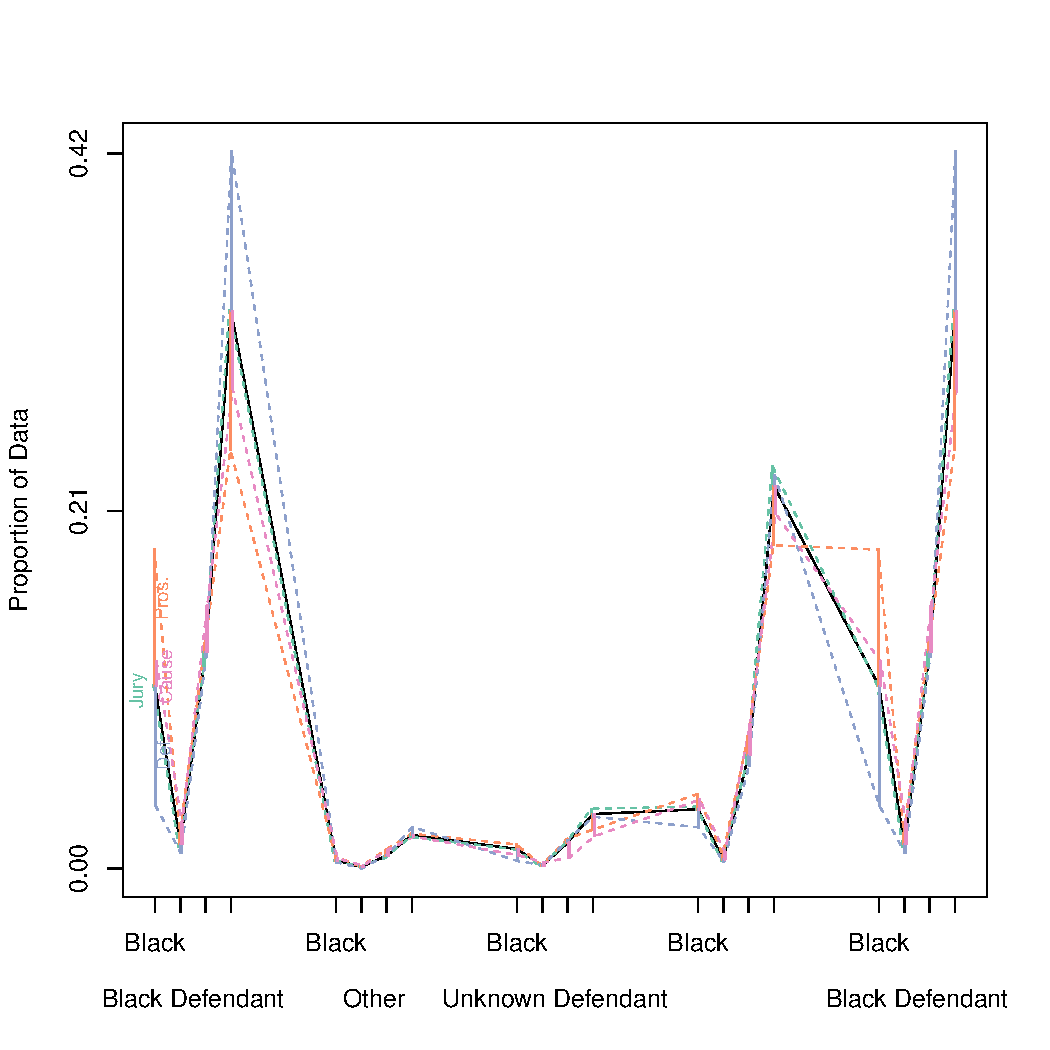
\includegraphics[width=0.7\textwidth]{FirstParCoord}
  \caption[First Parallel Coordinate Attempt]{\footnotesize The first attempt at a parallel coordinate plot. Note that the cramped
    display and unclear definition of the axis make interpretation even less intuitive than the mosaic plot, suggesting that this
    first attempt was a decided failure.}
  \label{fig:firstparcoord}
\end{figure}

Motivated by these concepts, parallel coordinates (as in \cite{wegman1990}) were used to visualize the data next, as can be seen
in Figure \ref{fig:firstparcoord}. This attempted visualization is arguably more difficult to interpret than the mosaic plot. It
is cluttered by the parallel coordinate lines, the bars emanating from each point obscure the fact that the end point of the bar
is the only feature of interest, and the meaning of the black reference line is entirely unclear without extensive
explanation. Finally, by viewing the distribution of each disposition, the wrong conditional density is being examined,
$P(Race,Race Defendant|Disposition)$. Multiple edits and re-conceptualizations of the concept eventually resulted in the ``mobile
plot,'' so-named due to its passing resemblance to the mobiles hung above babies' cribs.

An example of this plot can be seen in Figure \ref{fig:racedefmob}. Note that this plot is less cluttered than either the mosaic plot or
the first parallel coordinate plot, despite displaying more information. It is also more efficient with data-ink, avoids
displaying data with higher dimensions than the data itself, and uses redundant encoding of information in visual cues which are
high in the hierarchy presented by \cite{cleveland1987}. These redundancies include using both colour and ordering to represent
the different dispositions; and using both position along a common scale and length to communicate the conditional probabilities
of each disposition.

An explanation of the features and encoding used in the mobile plot is presented in \ref{app:mobile}.

\section{The Mobile Plot} \label{app:mobile}

The mobile plot consists of multiple grouped vertical lines anchored at one end to horizontal black lines, and at the other to
points. Information is encoded using length, colour, and position relative to a common scale. The vertical axis is meant to show
the value of a continuous variable, while the horizontal axis shows the value of a, possibly hierarchical, categorical
variable. It can be used to display the relationship between three
categorical variables in a meaningful
two-dimensional plot.

To show the grouping of categories on the horizontal axis, position is used. Those categorical levels which are grouped by some
separate categorical variable are placed closer to each other than those which are not in the same group. Each categorical
variable combination corresponds to a single horizontal black line, the length of which is proportional to the count of the
associated combination in the data being plotted. The vertical position of this line corresponds to the value of the continuous
variable expected for that particular combination.

Each of the vertical lines which extend from this horizontal line corresponds to a particular value of a third categorical
variable, coloured to show the specific level across the different horizontal lines. The end points of these lines represent the
observed distribution of the third variable for the two way
combination of the first two variables associated with the horizontal
line to which the points are attached. The lengths of these lines correspond to the deviation of the observation from the expectation. If a
different expectation is desired for the different values of the third categorical variable, the horizontal lines can be split
evenly and placed vertically at this expectation, to the detriment of grouping clarity.

In the case that such a split is not used and the continuous variable is the probability of a particular value of the third
categorical variable given the first two, the plot serves as a visual test of a very specific hypothesis: that of a uniform
distribution of the third categorical variable with respect to the two variables represented horizontally. Such a plot is powerful
because it allows for the simple detection of main effects and interaction effects over the three categorical variables against
this hypothesis.